%\chapter{Implementation}\label{s:implementation}
%\graphicspath{ {./images/} }
%\begin{figure}[t]
%\centering
%\caption{Zoomed in on QAS of ASR-1}
%\label{fig:ASR2}
%\end{figure}
%\includegraphics[width=12cm]{Decomposition of ASR and QAS_zoomed in on %ASR-1 and ASR-2_v2.jpg}\\
\chapter{Implementation}\label{s:Implementation}
\todo{better describe why there is a different between currently implemented and future architectures}
To answer research question 2 and combining it with the answer of research question 3 in context of software architecture, it can be explained in architectural patterns and tactics. Bass \etal \cite{Bass2015SoftwareAI} describes architectural patters as "Compositions of architectural elements and provide packaged strategies for solving some of the problems facing a system."

Patterns exist of multiple tactics. While tactics are chosen to empower a single quality attribute, a pattern could serve multiple quality attributes. This chapter will cover one pattern and a set of tactics. Both focused on the quality attribute of confidentiality.
\footnote{This research covers only one pattern and a few tactics. Specialists like cryptographers could argue there is an extensive set of patterns and tactics that can be applied.}

\section{Greenfield solutions - newly implemented architectures}
\subsection{Pattern - Apply Zero-knowledge proof}
\graphicspath{ {./images/} }
\begin{figure}[t]
\centering
\label{fig:ZKP}
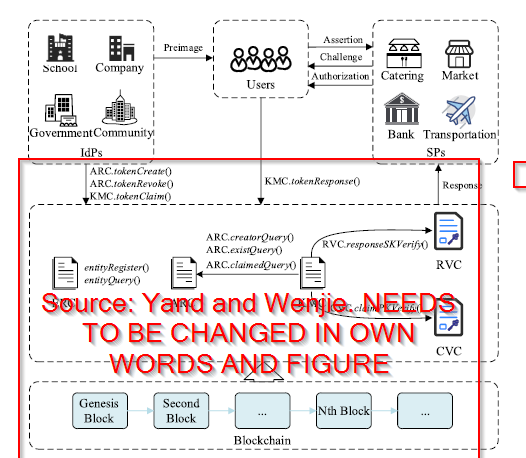
\includegraphics[width=16cm]{A zero-knowledge-proof-based digital identity management scheme in blockchain.png}\\
\caption{Zero knowledge proof}
\end{figure}

Xiaohui Yang and Wenjie Li\cite{YANG2020102050} state "Zero-knowledge proof (ZKP) is a cryptographic technique,
which means that the prover can convince the verifier that a certain statement is correct without providing the verifier with any additional information or leaking any information about the witness." The paper shows a method on how to implement Zero-knowledge proof without exposing personal information of the subject. Figure 5.2 shows a schema on how this principle works. Basically it means the party requesting information does not get all data, but only an answer on its question.

\subsection{Trade-offs and concerns}
Firstly, this method is based on blockchain technology, meaning this pattern is suitable in online scenarios. Secondly, blockchain technology is relatively new and knowledge on this topic can be scarce. Both are a trade-off to take in account when applying this pattern. 
\todo{Better describe and support these trade-offs and concerns}

\section{Brownfield solutions - currently used architectures }
\subsection{Confidentiality tactics}
\graphicspath{ {./images/} }
\begin{figure}[t]
\centering
\label{fig:Tactics}
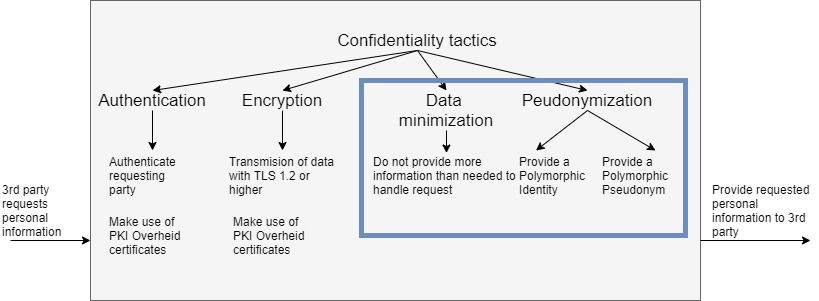
\includegraphics[width=17cm]{Tactics.jpg}\\
\caption{Confidentiality tactics}
\end{figure}

\subsection{Authentication}
A commonly used method for authentication purposes is usage of a certificate. For parties who communicate with on or on behalf of the Dutch government the government issues PKIoverheid (PKIO) certificates. These certificates are used for Authentication, Electronic signatures and encryption. \cite{Logius_PKIO}

\subsection{Data minimization}
\todo{add a description of this method, but emphasise how it's possible to use in software architecture}
\lipsum[1-1]

\subsection{Encryption - Transfer of data is encrypted with TLS 1.2 or higher}
A broadly implemented standard. The Dutch government has a reference architecture NORA (Nederlandse Overheid Referentie Architecture) \cite{NORA} which states this standard needs to be applied or otherwise explained why it has not been implemented \cite{NORA_PasToeOfLegUit}. On the part of TLS its clear version 1.2 or higher is accepted, but version 1.3 is prefered \cite{NORA_TLS}. 

\subsection{Peudonymization - Polymorphic Identity or Polymorphic Pseudonym}
When it's mandatory to share personal information, because it's for example mandatory by law, it's possible to provide this information as a pseudonym. GDPR \cite{GDPR} defines this method as a possibility to mitigate unwanted disclosure of personal information. 
This technique is already implemented and proven it can work by Erik Verheul \cite{VerheuleID}. 

%%% Local Variables:
%%% mode: latex
%%% TeX-master: "../thesis"
%%% End:
